%!TEX root = ../thesis.tex
% ******************************* Thesis Appendix B ********************************

% **************************** Define Graphics Path **************************
\ifpdf
    \graphicspath{{content/appendix3/figs/raster/}{content/appendix3/figs/pdf/}{content/appendix3/figs/}}
\else
    \graphicspath{{content/appendix3/figs/vector/}{content/appendix3/figs/}}
\fi


\chapter{Case Study 2: Seasonal Variations in Macroplastic Distributions}

\begin{figure}
    \centering
    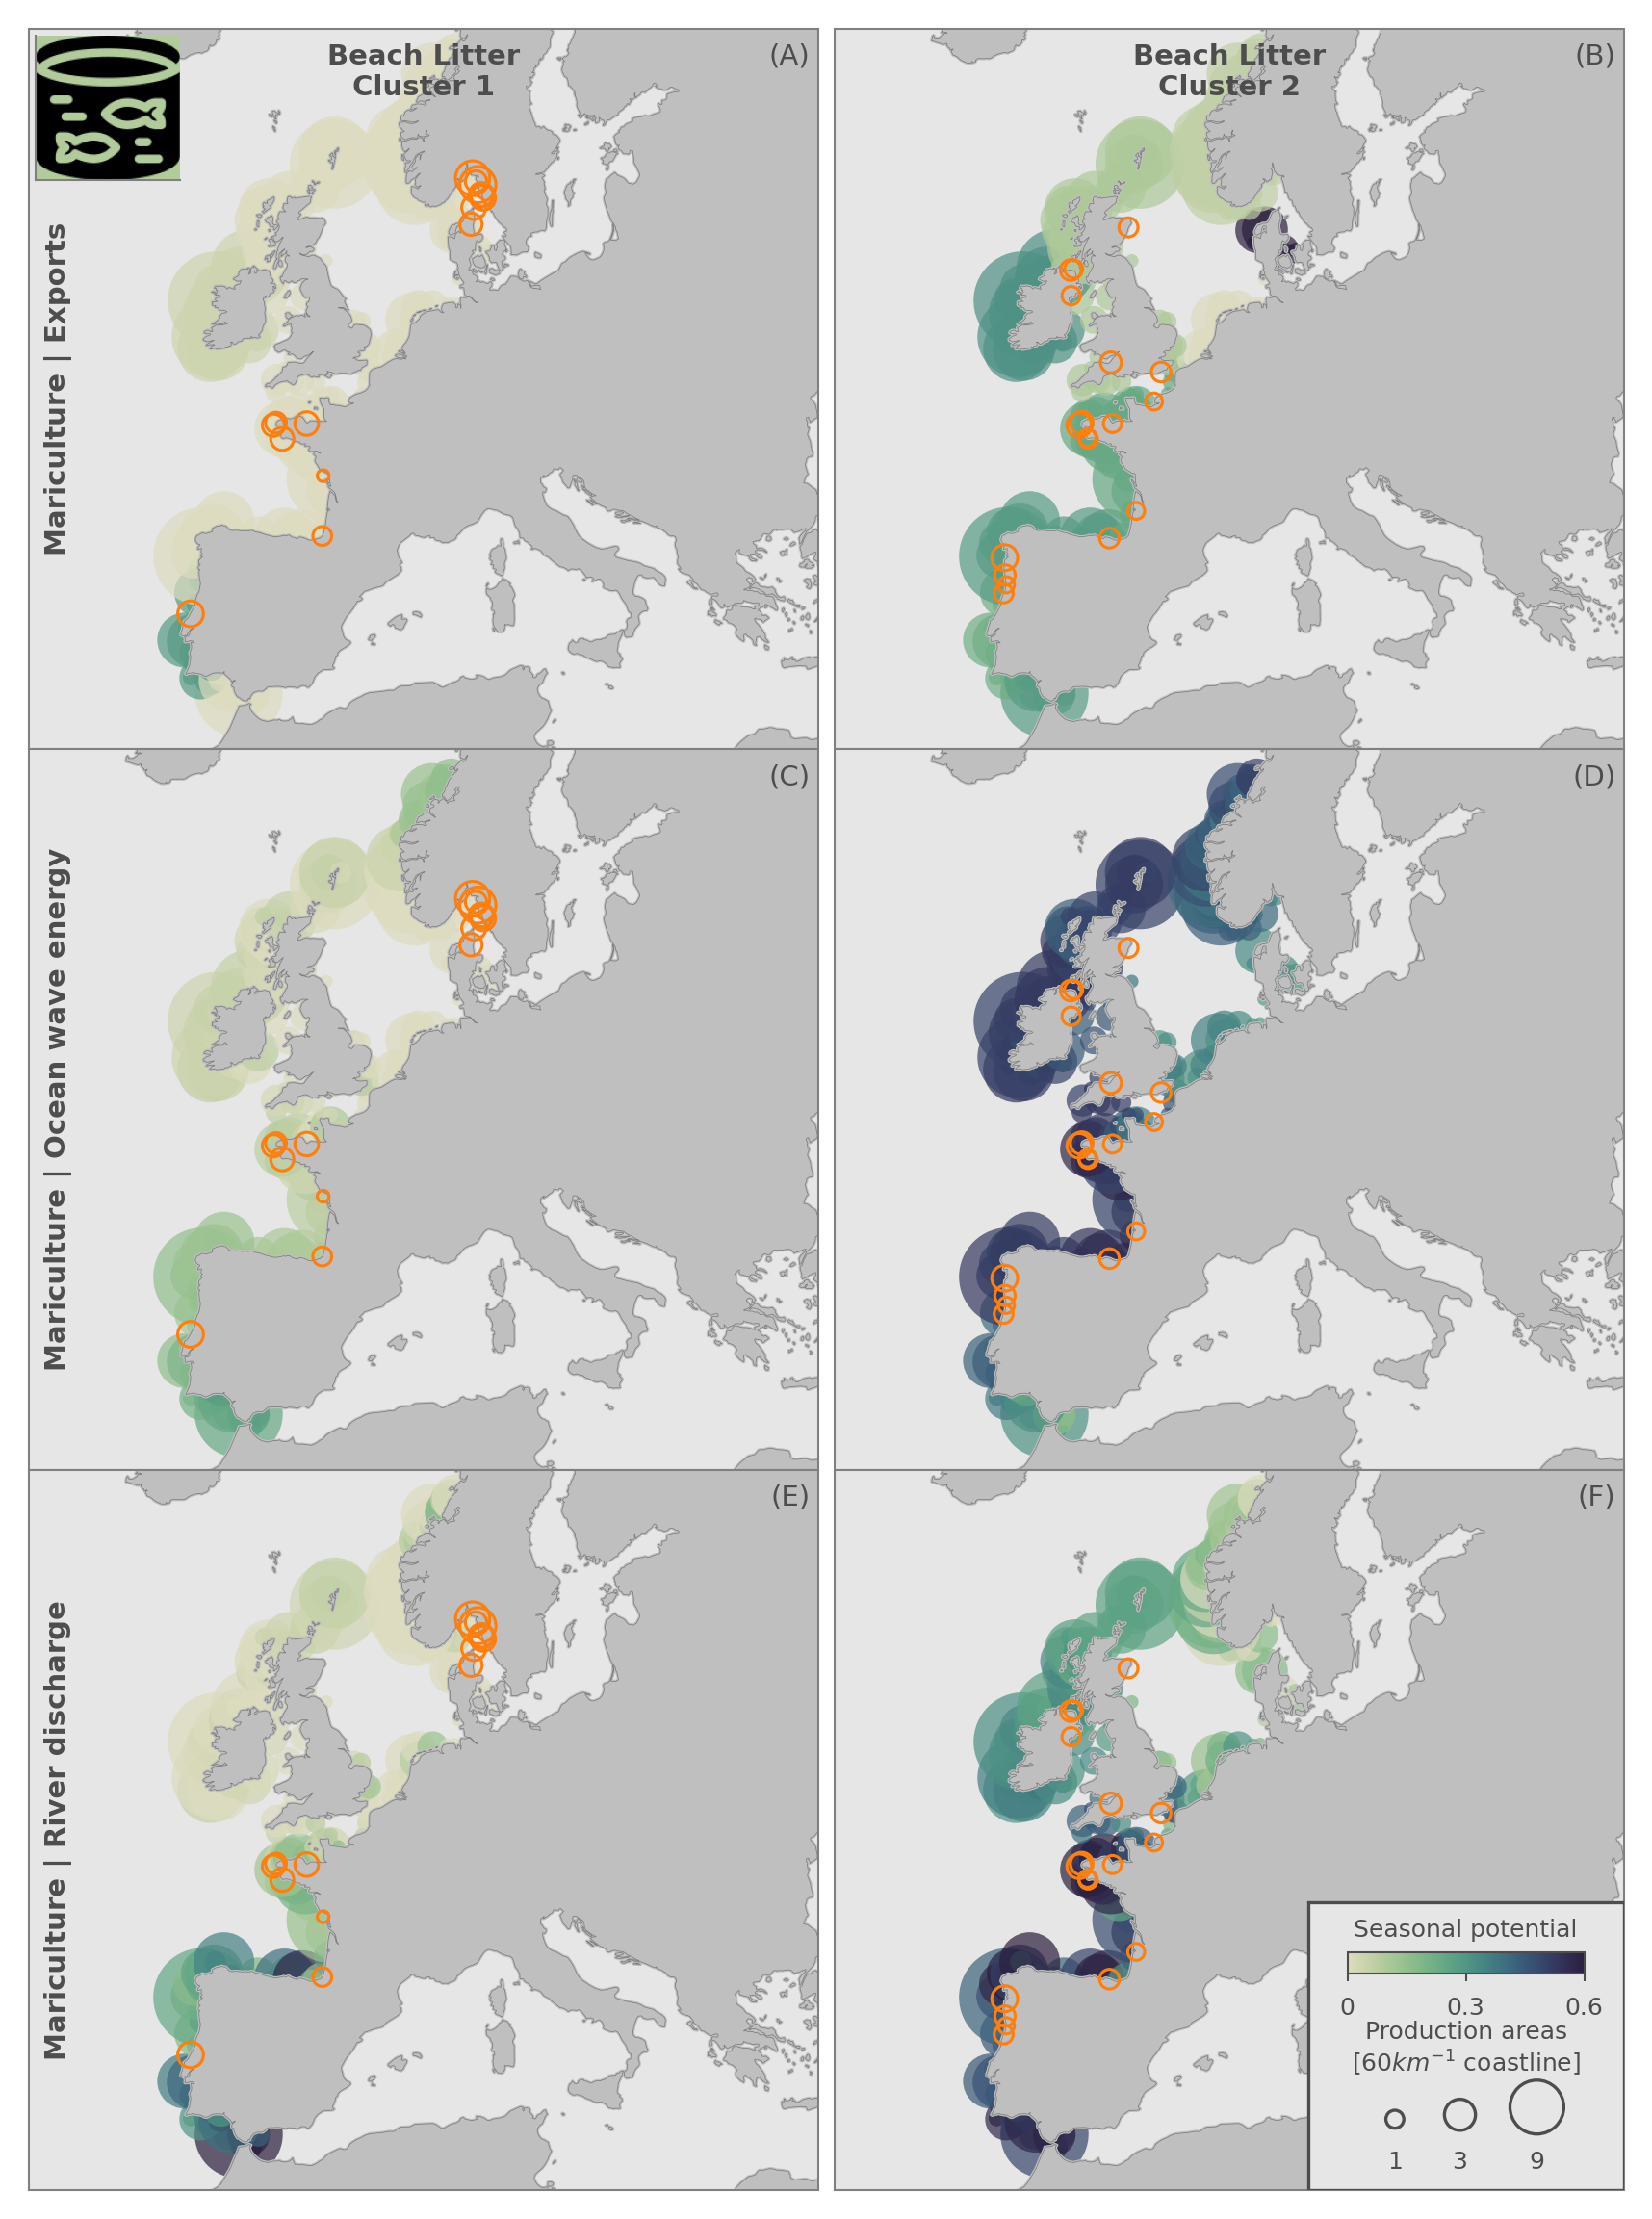
\includegraphics[width=0.95\textwidth]{plastics_seasonal_potential_mariculture}
    \caption[Seasonal potential of mariculture for seasonal beach litter patterns.]{\textbf{Seasonal potential of mariculture for seasonal beach litter patterns.} This figure parallels Figure~\ref{fig:plastics:seasonal_potential_map}, with rows illustrating different scenarios based on various drivers of mariculture macroplastic emissions (see Methods in the main text). \textbf{(A, B)} The first row uses exports of mariculture products as a proxy for peak activity during harvest periods. \textbf{(C, D)} The second row represents ocean wave energy as a proxy for adverse weather conditions. \textbf{(E, F)} The third row employs river discharge as a proxy for wear and tear intensity at mariculture sites located in river mouths. Reproduced with permission from Springer Nature.}
    \label{fig:plastics:seasonal_potential_mariculture_map}
\end{figure}

\begin{figure}
    \centering
    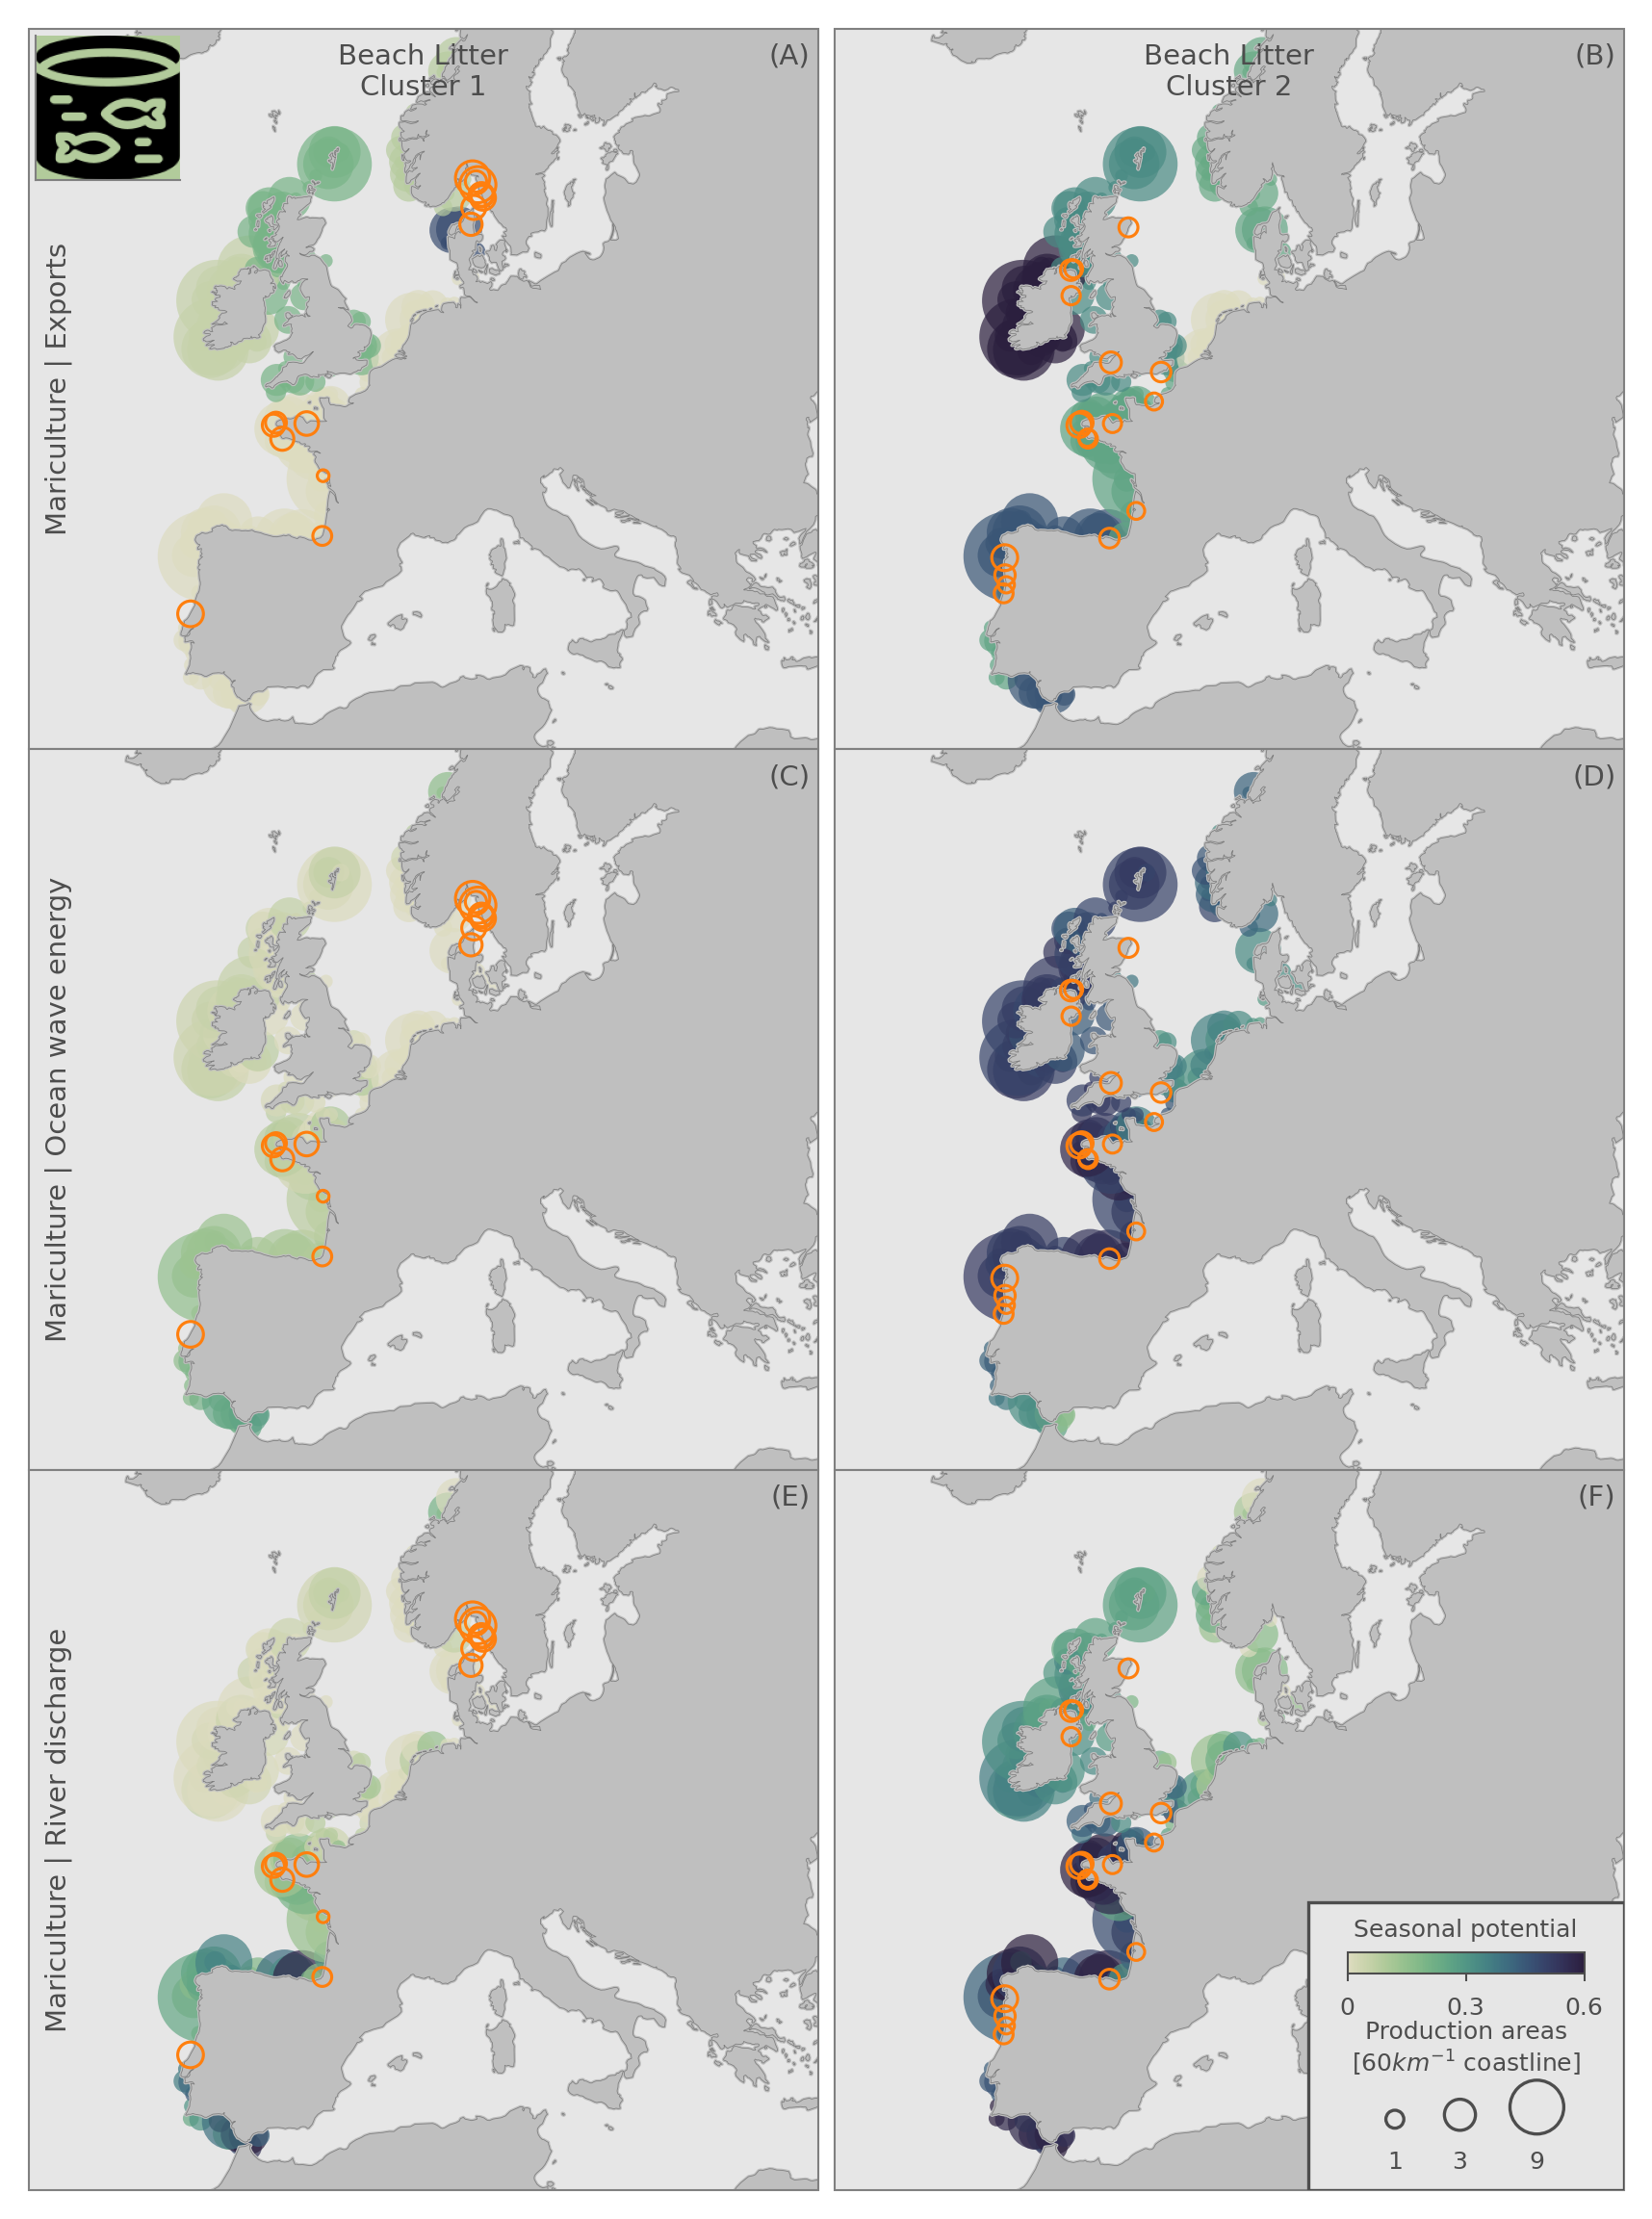
\includegraphics[width=0.95\textwidth]{plastics_seasonal_potential_mariculture_bivalve}
    \caption[Seasonal potential of mussel and oyster production for seasonal beach litter patterns]{\textbf{Seasonal potential of mussel and oyster production for seasonal beach litter patterns.} This figure is analogous to Figure~\ref{fig:plastics:seasonal_potential_mariculture_map}, but it focuses specifically on mussel and oyster production instead of all mariculture activities. Reproduced with permission from Springer Nature.}
    \label{fig:plastics:seasonal_potential_bivalve_map}
\end{figure}


\begin{figure}
    \centering
    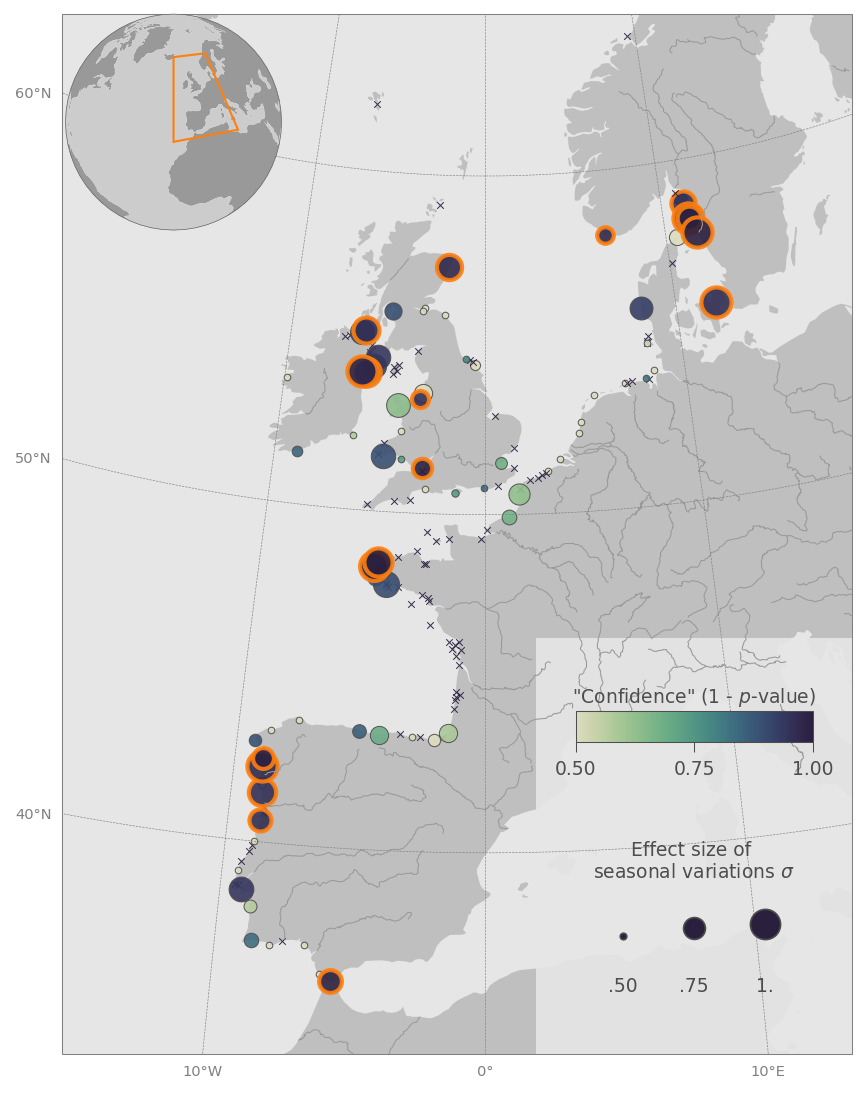
\includegraphics[width=0.95\textwidth]{plastics_seasonality_map_isolated}
    \caption[Seasonal variations in macroplastic distributions via a non-Bayesian approach.]{\textbf{Seasonal variations in macroplastic distributions via a non-Bayesian approach.} Seasonal variations were analyzed using a non-Bayesian method that excludes data from adjacent beaches, in contrast to the procedure presented in Figure~1 of the main text. A Kruskal-Wallis test was applied to four seasonal groups to detect variations, requiring at least 5 samples in no fewer than 2 groups to ensure adequate test power. Beaches that failed to meet this criterion are marked with a cross. Pairwise Mann-Whitney U tests were then conducted to identify significant seasonal differences, with p-values adjusted using the Benjamini-Hochberg correction for multiple comparisons. Results revealed that 20 beaches (\qty{11.9}{\percent} of the total) exhibit significant seasonal variation (p $< 0.05$), indicated by red edge colors in plots of 1 minus the p-value. Effect sizes were evaluated using the maximum biserial rank correlation across seasonal combinations for each beach, enabling direct comparison with the results presented in Figure~\ref{fig:plastics:seasonality_map_lgcp}. Reproduced with permission from Springer Nature.}
    \label{fig:plastics:seasonality_map_isolated}
\end{figure}